

\begin{comment}
\begin{figure*}[ht]
\centering
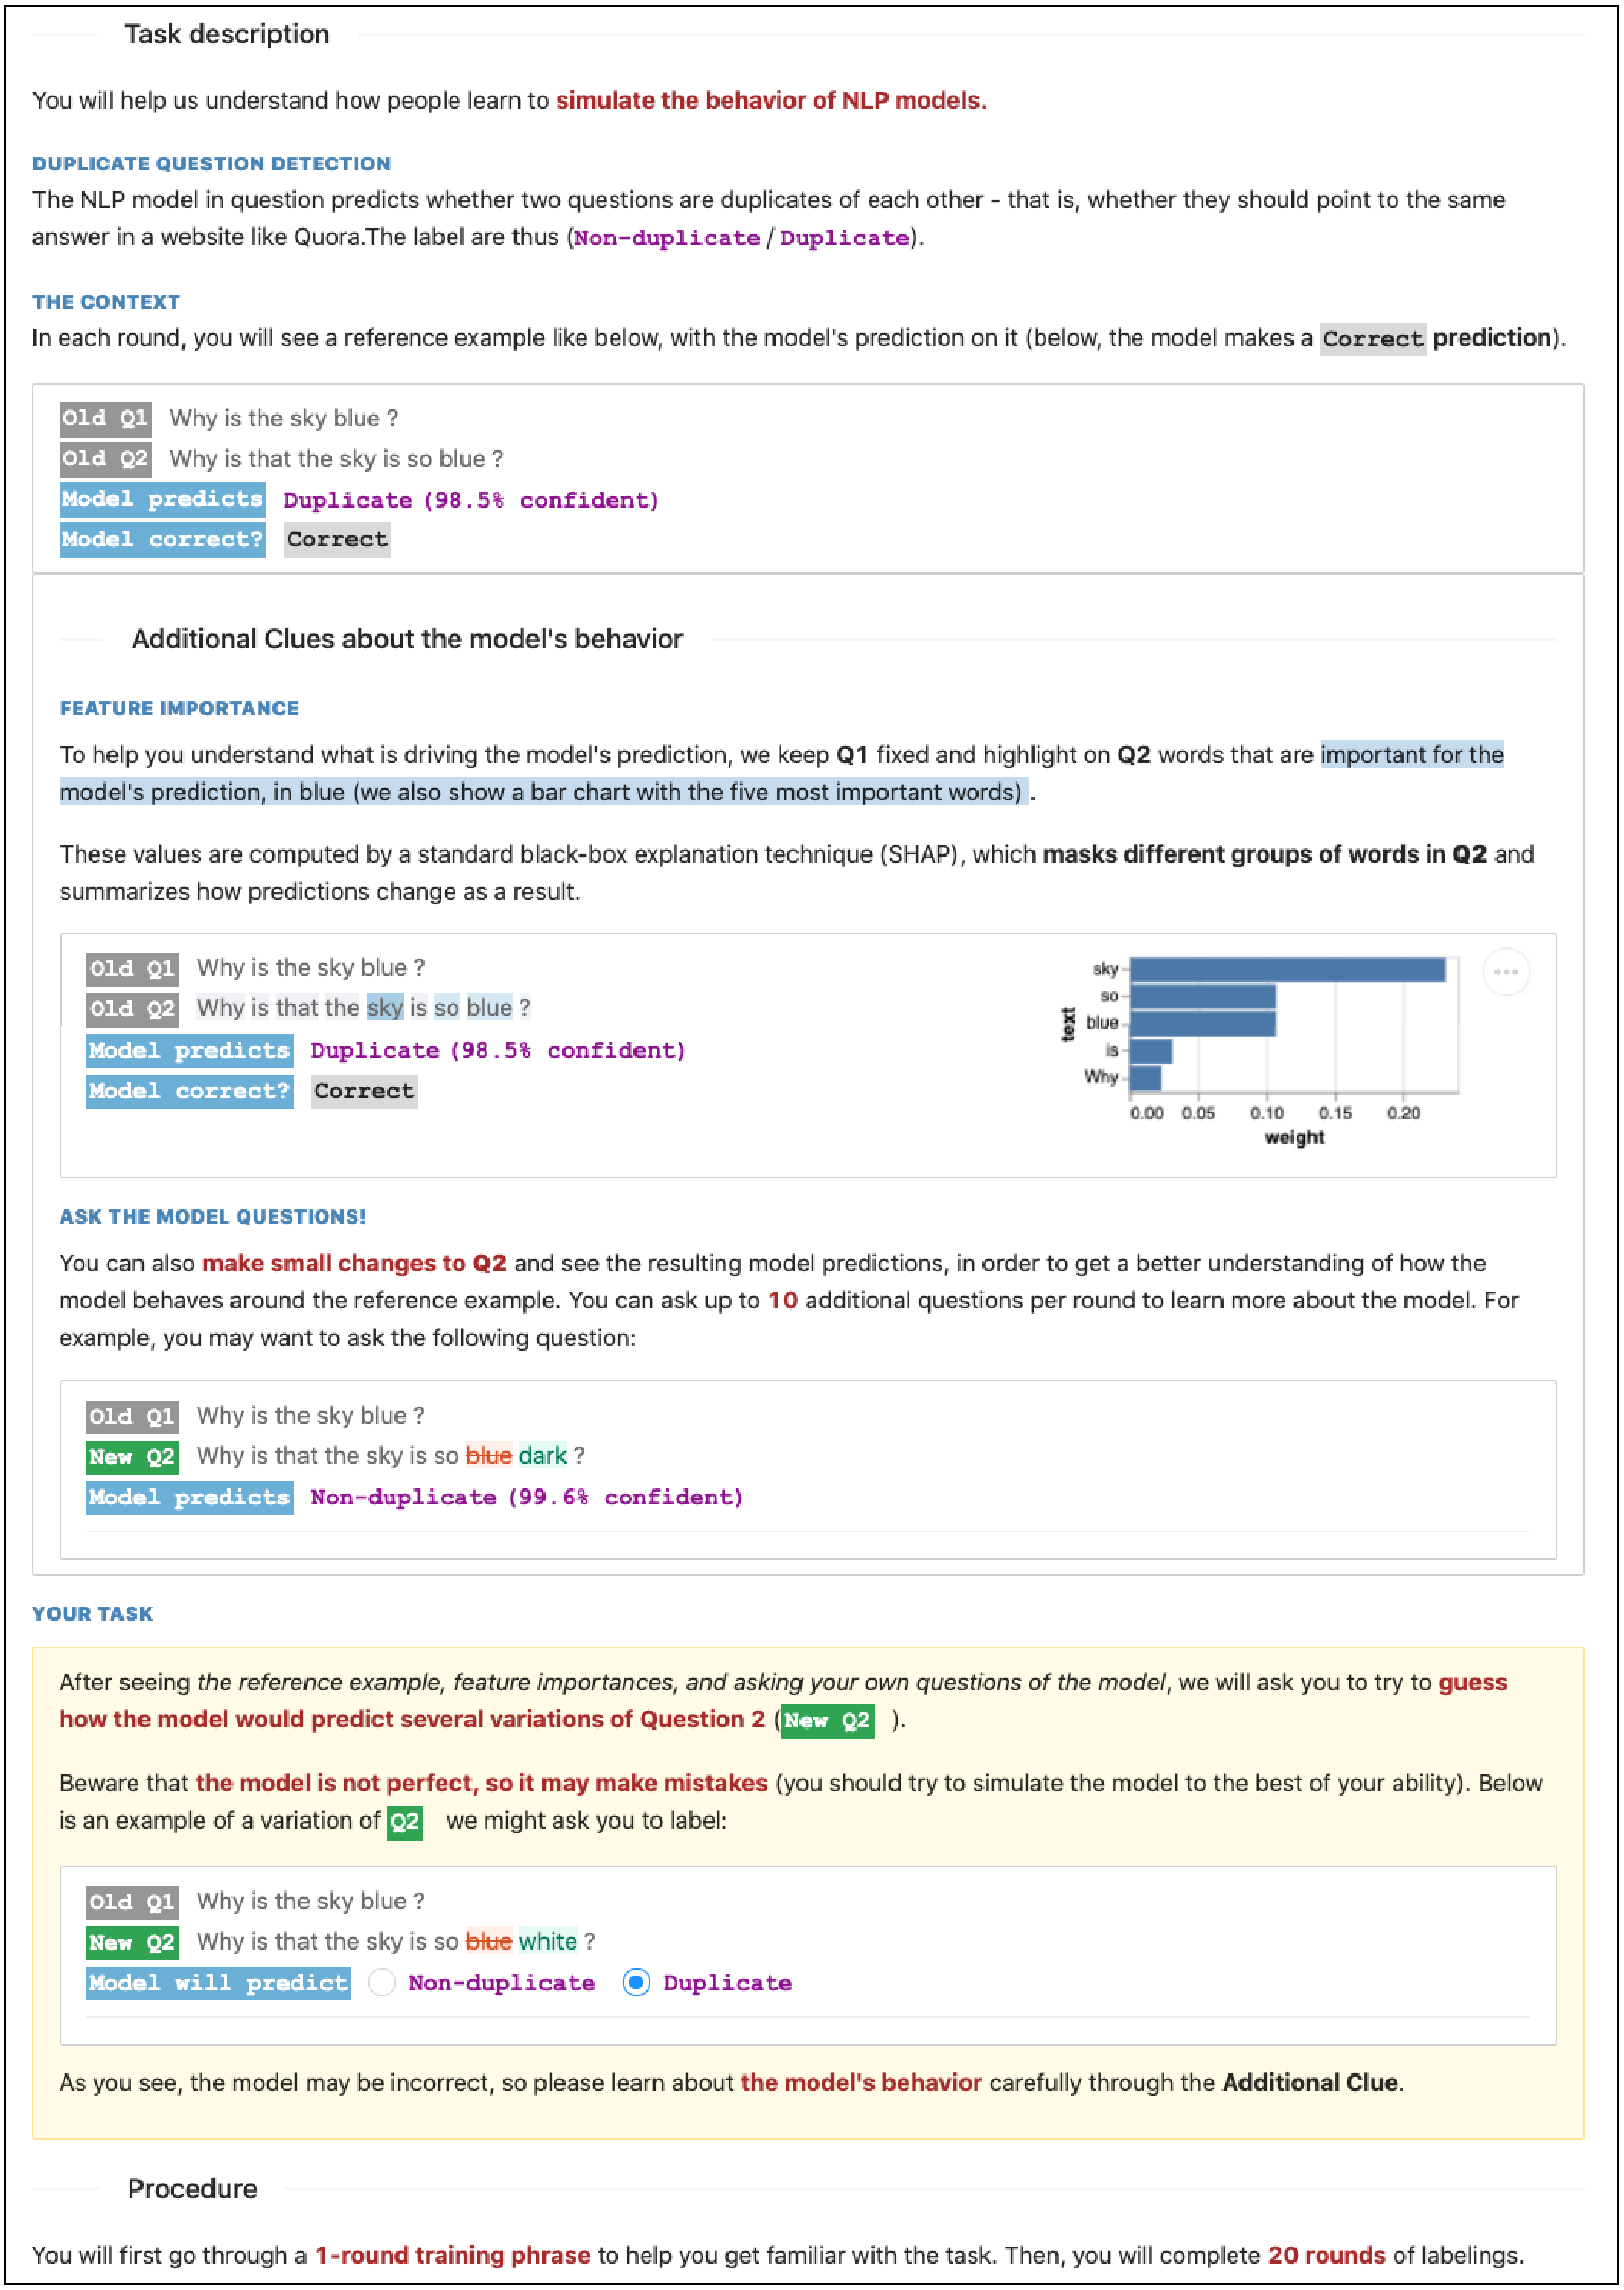
\includegraphics[width=1\textwidth]{figures/explanation_instruction}
\vspace{-15pt}
\caption{The instruction for the explanation study in \S\ref{subsec:exp_user_study}. \wts{Maybe remove.}}
\vspace{-10pt}
\label{fig:explanation_instruction}
\end{figure*}
\end{comment}

\begin{figure*}[ht]
\centering
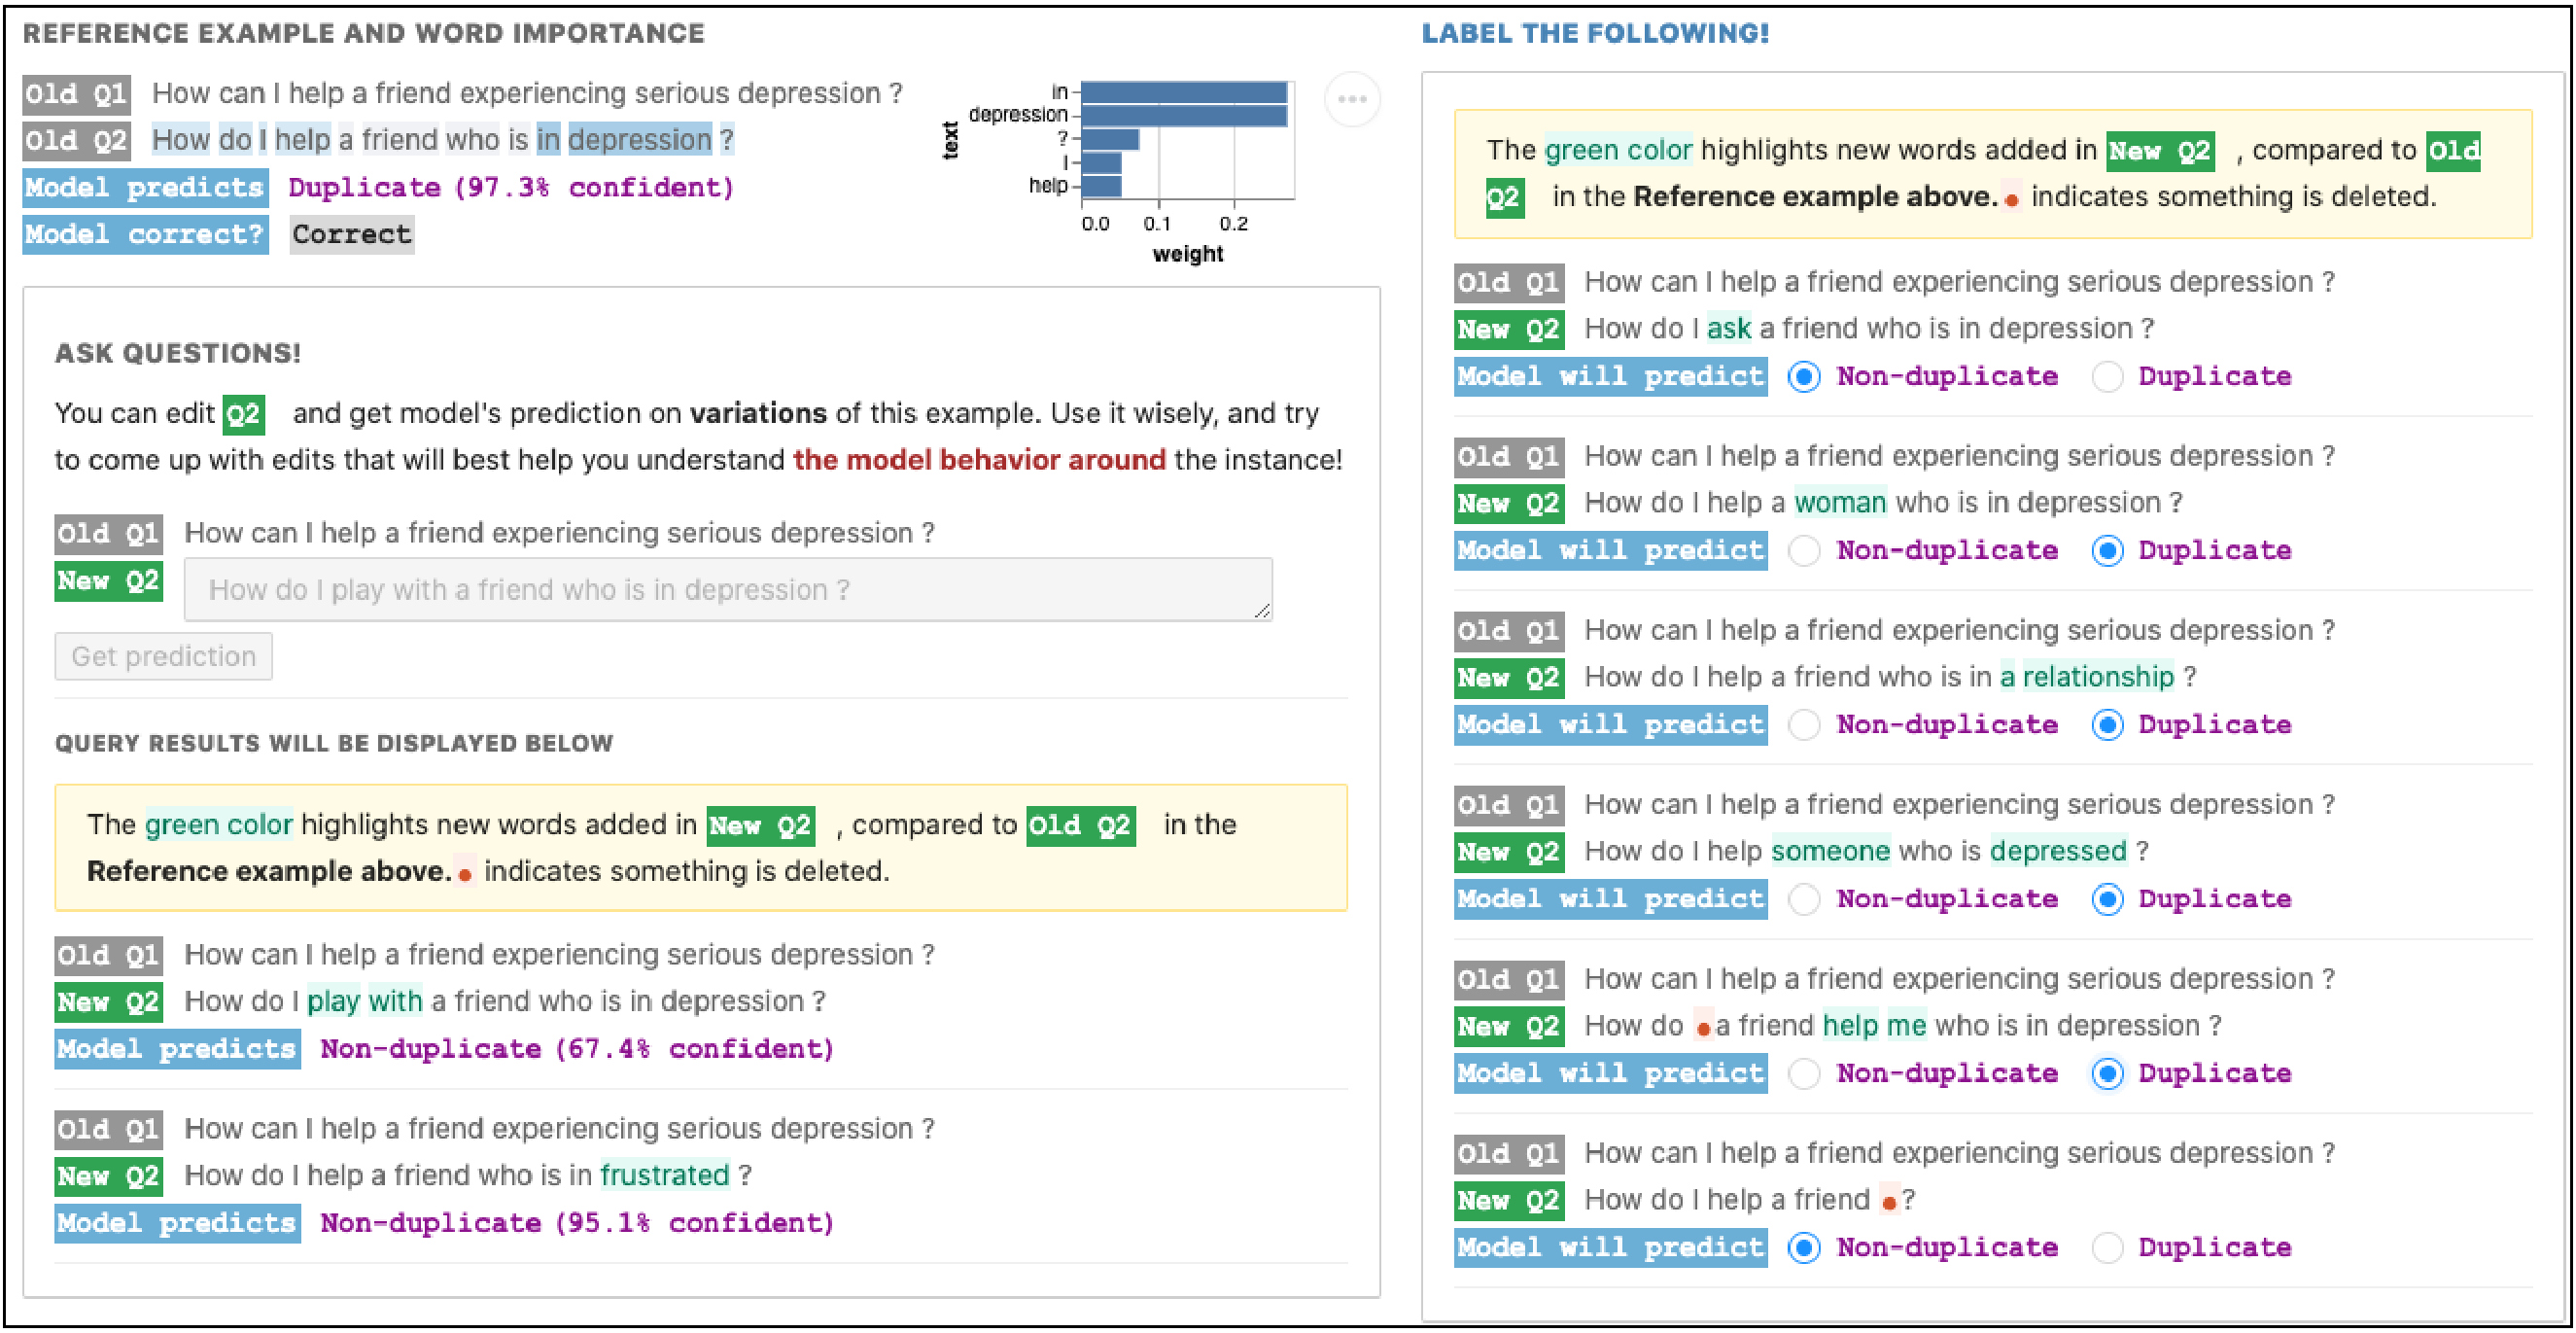
\includegraphics[width=0.85\textwidth]{figures/explanation_task_ui}
\vspace{-5pt}
\caption{A sample explanation task for \S\ref{sec:app_explain}}
\vspace{-10pt}
\label{fig:explanation_ui}
\end{figure*}

\section{Additional Explanation Details \S\ref{sec:app_explain}}
\label{appendix:explanation}


\subsection{Selection Methods}
\label{appendix:exp_rank}

Because  SHAP weights reflect the average effect of masking a token $t$, we also focus on \emph{word features that are abnormal on average}.

More concretely, we define the expected change-in-prediction for perturbing a token $t$ to be the SHAP importance on it, $\E[\dist(t, x)] = s(t)$.
In Figure~\ref{fig:explanation}, $s(t\text{=\remove{depression}})=0.276$.
The actual prediction change $\dist(t, x)$ is the weighted average of $|\fp(x)-\fp(\xp)|$ for all the $\xp$ that affect $t$ (\swap{depression}{trouble}, \swap{depression}{a mood}), where $\fp(x)$ is the prediction probability of $f$ on $x$.
The weight corresponds to the number of words modified in $\xp$: If $e(\xp)$ denotes the set of edited words in $x$, then $w(\xp) = 1/|e(\xp)|$.
Intuitively, the more words changed in $\xp$, the less impact each word has; In Figure~\ref{fig:explanation}D, we regard ``depression'' to be responsible for half of the impact in \swap{in depression}{suicidal}.
We group $\xp$ based on their affected words $G_t = \{\xp\ |\ t \in e(\xp)\}$. $\dist(t, x)$ then becomes:
$$\dist(t, x) = \frac{1}{|G_t|+1} \left(s(t) + \sum_{\xp \in G_t} w(t)\cdot |\fp(x)-\fp(\xp)|\right)$$
The additional SHAP weight $s(t)$ acts as a smoothing factor to penalize outliers.
Then the gap between the expectation and reality is:
$$\Delta\dist(t, x) = \dist(t, x)-\E[\dist(t, x)]$$
We first find the abnormal tokens: (1) $t$ with small SHAP weight, but $\xp$ that change $t$ experience large prediction change on average: $t_L = \argmax_{t\in x} \Delta\dist(t, x)$, and (2) $t$ with large SHAP weight, but $\xp$ with $t$ changed usually have intact prediction: $t_U = \argmax_{t\in x} -\Delta\dist(t, x)$.

Then, we use the most extreme cases within the groups of $G_{t_L}$ and $G_{t_U}$ as the concrete counterfactual explanations, based on their prediction change $|\fp(x)-\fp(\xp)|$, and the aggregated SHAP weights of all the changed tokens:
$$\xp_L = \argmax_{\xp \in G_{t_L}} \left( |f_p(x)-f_p(\xp)| - \sum_{u\in r(\xp)} s(u) \right)$$ 


\subsection{User Study Details}
\label{appendix:exp_user_study}

%The instruction for the user study in \S\ref{subsec:exp_user_study} is in Figure~\ref{fig:explanation_instruction}, and 
Figure~\ref{fig:explanation_ui} shows the sample interface. 
Participants started by just seeing the reference example and the model query box on the left hand side.
When they chose to start the task or after they had exhausted their ten query chances, the query box was disabled, the tasks on the right were displayed, and the participants completed the tasks.
We compensated participants \$20 for the one hour study.
